\documentclass[aspectratio=169]{beamer}

% Theme and Color Setup
\usetheme{Madrid}
\usecolortheme{whale}
\useinnertheme{rectangles}
\useoutertheme{miniframes}

% Additional Packages
\usepackage[utf8]{inputenc}
\usepackage[T1]{fontenc}
\usepackage{graphicx}
\usepackage{booktabs}
\usepackage{listings}
\usepackage{amsmath}
\usepackage{amssymb}
\usepackage{xcolor}
\usepackage{tikz}
\usepackage{pgfplots}
\pgfplotsset{compat=1.18}
\usetikzlibrary{positioning}
\usepackage{hyperref}

% Custom Colors
\definecolor{myblue}{RGB}{31, 73, 125}
\definecolor{mygray}{RGB}{100, 100, 100}
\definecolor{mygreen}{RGB}{0, 128, 0}
\definecolor{myorange}{RGB}{230, 126, 34}
\definecolor{mycodebackground}{RGB}{245, 245, 245}

% Set Theme Colors
\setbeamercolor{structure}{fg=myblue}
\setbeamercolor{frametitle}{fg=white, bg=myblue}
\setbeamercolor{title}{fg=myblue}
\setbeamercolor{section in toc}{fg=myblue}
\setbeamercolor{item projected}{fg=white, bg=myblue}
\setbeamercolor{block title}{bg=myblue!20, fg=myblue}
\setbeamercolor{block body}{bg=myblue!10}
\setbeamercolor{alerted text}{fg=myorange}

% Set Fonts
\setbeamerfont{title}{size=\Large, series=\bfseries}
\setbeamerfont{frametitle}{size=\large, series=\bfseries}
\setbeamerfont{caption}{size=\small}
\setbeamerfont{footnote}{size=\tiny}

% Code Listing Style
\lstdefinestyle{customcode}{
  backgroundcolor=\color{mycodebackground},
  basicstyle=\footnotesize\ttfamily,
  breakatwhitespace=false,
  breaklines=true,
  commentstyle=\color{mygreen}\itshape,
  keywordstyle=\color{blue}\bfseries,
  stringstyle=\color{myorange},
  numbers=left,
  numbersep=8pt,
  numberstyle=\tiny\color{mygray},
  frame=single,
  framesep=5pt,
  rulecolor=\color{mygray},
  showspaces=false,
  showstringspaces=false,
  showtabs=false,
  tabsize=2,
  captionpos=b
}
\lstset{style=customcode}

% Custom Commands
\newcommand{\hilight}[1]{\colorbox{myorange!30}{#1}}
\newcommand{\source}[1]{\vspace{0.2cm}\hfill{\tiny\textcolor{mygray}{Source: #1}}}
\newcommand{\concept}[1]{\textcolor{myblue}{\textbf{#1}}}
\newcommand{\separator}{\begin{center}\rule{0.5\linewidth}{0.5pt}\end{center}}

% Footer and Navigation Setup
\setbeamertemplate{footline}{
  \leavevmode%
  \hbox{%
  \begin{beamercolorbox}[wd=.3\paperwidth,ht=2.25ex,dp=1ex,center]{author in head/foot}%
    \usebeamerfont{author in head/foot}\insertshortauthor
  \end{beamercolorbox}%
  \begin{beamercolorbox}[wd=.5\paperwidth,ht=2.25ex,dp=1ex,center]{title in head/foot}%
    \usebeamerfont{title in head/foot}\insertshorttitle
  \end{beamercolorbox}%
  \begin{beamercolorbox}[wd=.2\paperwidth,ht=2.25ex,dp=1ex,center]{date in head/foot}%
    \usebeamerfont{date in head/foot}
    \insertframenumber{} / \inserttotalframenumber
  \end{beamercolorbox}}%
  \vskip0pt%
}

% Turn off navigation symbols
\setbeamertemplate{navigation symbols}{}

% Title Page Information
\title[Week 9: Multi-Agent RL]{Week 9: Multi-Agent Reinforcement Learning}
\author[J. Smith]{John Smith, Ph.D.}
\institute[University Name]{
  Department of Computer Science\\
  University Name\\
  \vspace{0.3cm}
  Email: email@university.edu\\
  Website: www.university.edu
}
\date{\today}

% Document Start
\begin{document}

\frame{\titlepage}

\begin{frame}[fragile]
    \frametitle{Introduction to Multi-Agent Reinforcement Learning}
    \begin{block}{What are Multi-Agent Systems?}
        \begin{itemize}
            \item \textbf{Definition}: A multi-agent system (MAS) consists of multiple interacting agents (either cooperative or competitive) that work together or against each other to achieve specific goals in a shared environment.
            \item \textbf{Characteristics}:
            \begin{itemize}
                \item \textbf{Autonomy}: Agents operate independently.
                \item \textbf{Interaction}: Agents communicate and affect one another’s actions.
                \item \textbf{Learning}: Agents can learn and adapt based on experiences.
            \end{itemize}
            \item \textbf{Types of Agents}:
            \begin{itemize}
                \item Cooperative Agents: Work towards a common goal (e.g., robotic teams).
                \item Competitive Agents: Opposing each other's objectives (e.g., gaming scenarios).
            \end{itemize}
        \end{itemize}
    \end{block}
\end{frame}

\begin{frame}[fragile]
    \frametitle{Significance of Multi-Agent Reinforcement Learning}
    \begin{block}{Importance of MARL}
        \begin{itemize}
            \item \textbf{Complex Environments}: Real-world problems often involve multiple entities that influence one another, making single-agent approaches inadequate.
            \item \textbf{Learning Dynamics}: 
            \begin{itemize}
                \item With multiple agents, the environment becomes non-stationary since each agent’s actions impact the others, requiring continuous adaptation.
            \end{itemize}
            \item \textbf{Applications}:
            \begin{itemize}
                \item Robotics: Coordination of robotic teams for tasks like search and rescue.
                \item Negotiation Systems: Agents negotiating in economic scenarios to maximize profits or satisfaction.
                \item Game Playing: Advancements in AI for games like chess or poker that involve multiple players.
            \end{itemize}
        \end{itemize}
    \end{block}
\end{frame}

\begin{frame}[fragile]
    \frametitle{Key Points and Conclusion}
    \begin{block}{Key Points to Remember}
        \begin{enumerate}
            \item Agents in MARL adapt based on the actions and strategies of others, increasing the complexity of the learning algorithm.
            \item Types of Interactions:
            \begin{itemize}
                \item Cooperation enhances performance on shared tasks.
                \item Competition can lead to robustness, as agents learn to strategize against opponents.
            \end{itemize}
            \item Challenges in MARL:
            \begin{itemize}
                \item Credit Assignment Problem: Determining which agent's actions contribute to the team's overall success.
                \item Scalability: As the number of agents increases, so do the complications in learning algorithms and interactions.
            \end{itemize}
        \end{enumerate}
    \end{block}
    \begin{block}{Conclusion}
        Multi-Agent Reinforcement Learning expands the traditional reinforcement learning framework to accommodate scenarios involving multiple decision-makers, providing sophisticated tools for tackling challenges in various domains ranging from robotics to economics. Understanding its principles is essential for developing effective strategies in complex environments.
    \end{block}
\end{frame}

\begin{frame}[fragile]{Learning Objectives - Overview}
    This week's focus on Multi-Agent Reinforcement Learning (MARL) aims to enhance your understanding of collaborative and competitive interactions in reinforcement learning scenarios. By the end of this session, you will achieve the following learning objectives:
\end{frame}

\begin{frame}[fragile]{Learning Objectives - Part 1}
    \begin{enumerate}
        \item \textbf{Define Multi-Agent Systems:} 
        \begin{itemize}
            \item Understand the concept of a multi-agent system (MAS) and differentiate between cooperative, competitive, and mixed-mode strategies.
            \item \textit{Example:} In a player versus player game, agents are competitors. In a robotic swarm, agents work together towards a common goal.
        \end{itemize}
        
        \item \textbf{Identify Key Components:} 
        \begin{itemize}
            \item Recognize critical elements in multi-agent environments such as agents, environments, states, actions, and rewards.
            \item \textit{Example:} In an autonomous driving scenario with multiple vehicles, each vehicle (agent) navigates (action) while responding to other vehicles and traffic signals (environment).
        \end{itemize}
    \end{enumerate}
\end{frame}

\begin{frame}[fragile]{Learning Objectives - Part 2}
    \begin{enumerate}[resume]
        \item \textbf{Explore Learning Paradigms:} 
        \begin{itemize}
            \item Examine various learning paradigms in MARL such as centralized vs. decentralized learning, and their implications on efficiency and scalability. 
            \item \textit{Emphasis:} Centralized learning relies on a global view for decision-making, while decentralized approaches empower individual agents to learn and adapt independently.
        \end{itemize}
        
        \item \textbf{Discuss Challenges in MARL:} 
        \begin{itemize}
            \item Investigate common challenges faced in MARL, including non-stationarity, credit assignment, and scalability issues.
            \item \textit{Key Point:} Non-stationarity arises because the environment changes as each agent learns, making it difficult for agents to optimize their strategies effectively.
        \end{itemize}
        
        \item \textbf{Introduce Application Areas:}
        \begin{itemize}
            \item Highlight real-world applications of MARL in areas such as robotics, traffic management, and economics.
            \item \textit{Example:} Use of MARL for traffic light control systems where multiple lights (agents) coordinate to optimize traffic flow.
        \end{itemize}
    \end{enumerate}
\end{frame}

\begin{frame}[fragile]{Learning Objectives - Part 3}
    \begin{enumerate}[resume]
        \item \textbf{Implement MARL Algorithms:}
        \begin{itemize}
            \item Provide an understanding of popular algorithms such as Independent Q-Learning and MADDPG (Multi-Agent Deep Deterministic Policy Gradient) and how they can be applied in practical scenarios.
            \item \textit{Snippet:}
            \begin{lstlisting}[language=Python]
# Example of independent Q-learning update
Q[state, action] += alpha * (reward + gamma * max(Q[next_state]) - Q[state, action])
            \end{lstlisting}
        \end{itemize}
    \end{enumerate}
\end{frame}

\begin{frame}[fragile]{Key Takeaways}
    \begin{itemize}
        \item \textbf{Collaborative vs. Competitive Dynamics:} Understanding these dynamics is crucial for designing effective multi-agent systems.
        \item \textbf{Scalability and Coordination:} As the number of agents increases, maintaining effective communication and coordination becomes challenging.
        \item \textbf{Real-World Relevance:} MARL serves multiple industries, enhancing solutions in critical sectors.
    \end{itemize}

    By achieving these objectives, you will gain a comprehensive understanding of how multiple agents can learn and interact in complex environments, setting the stage for deeper exploration of specific algorithms and their applications in subsequent slides. 
\end{frame}

\begin{frame}[fragile]
    \frametitle{Key Concepts in Multi-Agent RL}
    \begin{block}{Introduction to Multi-Agent Reinforcement Learning (MARL)}
        MARL extends traditional reinforcement learning (RL) to scenarios with multiple agents interacting within a shared environment. Key concepts include:
    \end{block}
    
    \begin{itemize}
        \item Agents
        \item Environment
        \item States
        \item Actions
        \item Rewards
    \end{itemize}
\end{frame}

\begin{frame}[fragile]
    \frametitle{Key Concepts: Agents and Environments}
    \begin{block}{Agents}
        \begin{itemize}
            \item \textbf{Definition}: An entity that perceives its environment and takes actions to maximize cumulative rewards.
            \item \textbf{Example}: In a game of soccer, each player represents an agent.
        \end{itemize}
    \end{block}
    
    \begin{block}{Environment}
        \begin{itemize}
            \item \textbf{Definition}: The setting surrounding the agents; it includes dynamics and interaction rules.
            \item \textbf{Example}: In a board game, the board layout and rules dictate movement.
        \end{itemize}
    \end{block}
\end{frame}

\begin{frame}[fragile]
    \frametitle{Key Concepts: States, Actions, and Rewards}
    \begin{block}{States}
        \begin{itemize}
            \item \textbf{Definition}: Describes the current situation of the environment.
            \item \textbf{Example}: For self-driving cars, the state includes nearby vehicles and traffic signals.
        \end{itemize}
    \end{block}
    
    \begin{block}{Actions}
        \begin{itemize}
            \item \textbf{Definition}: Choices made by agents to influence the environment.
            \item \textbf{Example}: In a trading simulation, agents can buy, sell, or hold stocks.
        \end{itemize}
    \end{block}

    \begin{block}{Rewards}
        \begin{itemize}
            \item \textbf{Definition}: Feedback signals given to agents after taking actions.
            \item \textbf{Example}: In a video game, a reward may be given for defeating an opponent.
        \end{itemize}
    \end{block}
\end{frame}

\begin{frame}[fragile]
    \frametitle{Interaction Dynamics in MARL}
    \begin{block}{Types of Interaction}
        \begin{itemize}
            \item \textbf{Cooperative}: Agents work together towards a common goal.
            \item \textbf{Competitive}: Agents compete against each other to succeed.
            \item \textbf{Mixed}: A combination of cooperation and competition.
        \end{itemize}
    \end{block}
    
    \begin{block}{Key Points to Emphasize}
        \begin{itemize}
            \item \textbf{Interdependence}: The success of one agent depends on the actions of others.
            \item \textbf{Adaptability}: Agents must adapt strategies as they learn from the environment.
        \end{itemize}
    \end{block}
\end{frame}

\begin{frame}[fragile]
    \frametitle{Conclusion and Code Snippet}
    \begin{block}{Conclusion}
        Understanding the key concepts in MARL is essential for analyzing and designing complex multi-agent systems.
    \end{block}
    
    \begin{block}{Optional Code Snippet}
        \begin{lstlisting}[language=Python]
import gym
import numpy as np

class MultiAgentEnv:
    def __init__(self, num_agents):
        self.num_agents = num_agents
        self.state = np.zeros((num_agents,))  # Shared state

    def step(self, actions):
        rewards = []
        for action in actions:
            rewards.append(action)  # Simple reward logic
        return self.state, rewards

env = MultiAgentEnv(num_agents=3)
        \end{lstlisting}
    \end{block}
\end{frame}

\begin{frame}[fragile]
    \frametitle{Types of Multi-Agent Systems}
    \begin{block}{Introduction}
        Multi-Agent Systems (MAS) can be classified based on the nature of the interactions between agents. Understanding these classifications is essential for designing effective multi-agent reinforcement learning (MARL) systems and addressing the unique challenges they present.
    \end{block}
\end{frame}

\begin{frame}[fragile]
    \frametitle{Cooperative Multi-Agent Systems}
    \begin{itemize}
        \item \textbf{Definition}: Agents work together towards a common goal, sharing knowledge and resources to maximize a joint reward.
        \item \textbf{Key Characteristics}:
            \begin{itemize}
                \item Collective reward for agents.
                \item Emphasis on communication and coordination.
            \end{itemize}
        \item \textbf{Examples}:
            \begin{itemize}
                \item Robotic Swarms: Drones coordinating for surveillance.
                \item Team Sports: Players coordinating to score points (e.g., basketball).
            \end{itemize}
        \item \textbf{Illustration}: An orchestra where each musician plays a different instrument to create harmonious music.
    \end{itemize}
\end{frame}

\begin{frame}[fragile]
    \frametitle{Competitive and Mixed Multi-Agent Systems}
    \begin{itemize}
        \item \textbf{Competitive Multi-Agent Systems}:
            \begin{itemize}
                \item \textbf{Definition}: Agents operate under opposing interests, vying for individual rewards.
                \item \textbf{Key Characteristics}:
                    \begin{itemize}
                        \item Adversarial nature; trying to outperform others.
                        \item Outcome for one agent typically results in loss for others.
                    \end{itemize}
                \item \textbf{Examples}:
                    \begin{itemize}
                        \item Game Theory: Chess competing against each other.
                        \item Economics: Companies competing for customers.
                    \end{itemize}
                \item \textbf{Illustration}: A race where runners strive to outpace each other, with only one winning.
            \end{itemize}
    \end{itemize}

    \begin{itemize}
        \item \textbf{Mixed Multi-Agent Systems}:
            \begin{itemize}
                \item \textbf{Definition}: Systems that have both cooperative and competitive elements.
                \item \textbf{Key Characteristics}: Complex interactions, balancing collaboration and competition.
                \item \textbf{Examples}:
                    \begin{itemize}
                        \item Market Trading: Traders collaborate for information but compete for profits.
                        \item Multi-Player Video Games: Teams may work together while having individual scores.
                    \end{itemize}
                \item \textbf{Illustration}: Community sharing resources to improve their environment while competing for limited grants.
            \end{itemize}
    \end{itemize}
\end{frame}

\begin{frame}[fragile]
    \frametitle{Conclusion and Key Points}
    \begin{block}{Conclusion}
        Understanding the types of multi-agent systems—cooperative, competitive, and mixed—enables better modeling of interactions in MARL environments. Each type presents different dynamics and challenges affecting strategy formulation and learning processes.
    \end{block}

    \begin{itemize}
        \item \textbf{Key Points to Emphasize}:
            \begin{itemize}
                \item Cooperative systems enhance synergy among agents.
                \item Competitive systems highlight strategic decision-making.
                \item Mixed systems require adaptability in cooperation and competition.
            \end{itemize}
    \end{itemize}
    
    \begin{block}{Additional Note}
        Formulating strategies in mixed systems may involve developing algorithms that dynamically switch between cooperative and competitive behaviors based on the context.
    \end{block}
\end{frame}

\begin{frame}[fragile]
    \frametitle{Challenges in Multi-Agent Reinforcement Learning - Non-Stationarity}
    \begin{itemize}
        \item \textbf{Explanation:} In a multi-agent environment, each agent adapts its strategy while others are learning, creating a non-stationary environment.
        \item \textbf{Example:} In chess, players adapt their strategies based on each other's moves, causing optimal strategies to change over time.
        \item \textbf{Impact:} Difficulty in policy convergence complicates the learning of stable strategies.
    \end{itemize}
\end{frame}

\begin{frame}[fragile]
    \frametitle{Challenges in Multi-Agent Reinforcement Learning - Credit Assignment Problem}
    \begin{itemize}
        \item \textbf{Explanation:} Outcomes depend on the actions of multiple agents, making it difficult to determine who is responsible for rewards, especially with delayed feedback.
        \item \textbf{Example:} In a team of robots, knowing each robot’s contribution to a task can be challenging if rewards are shared.
        \item \textbf{Solutions:}
        \begin{itemize}
            \item Design individual rewards for contributions.
            \item Use temporal difference methods or eligibility traces.
        \end{itemize}
    \end{itemize}
\end{frame}

\begin{frame}[fragile]
    \frametitle{Challenges in Multi-Agent Reinforcement Learning - Scalability}
    \begin{itemize}
        \item \textbf{Explanation:} Increasing the number of agents raises interaction complexity exponentially, complicating communication and computation.
        \item \textbf{Example:} Coordinating thousands of vehicles in traffic management presents significant decision-making challenges.
        \item \textbf{Impact:} Results in higher dimensional state spaces and the curse of dimensionality, making learning impractical without efficient methods.
    \end{itemize}
\end{frame}

\begin{frame}[fragile]
    \frametitle{Key Points and Conclusion}
    \begin{itemize}
        \item \textbf{Dynamic Interaction:} Agents must adapt to each other's actions as well as the environment.
        \item \textbf{Learning Strategies:} Strategies must balance cooperation and competition.
        \item \textbf{Algorithmic Innovation:} Novel algorithms are necessary to manage complexity and improve learning efficiency.
    \end{itemize}

    \textbf{Conclusion:} Understanding challenges in non-stationarity, credit assignment, and scalability is essential for developing effective multi-agent reinforcement learning systems.
\end{frame}

\begin{frame}[fragile]
    \frametitle{Multi-Agent Learning Frameworks - Overview}
    \begin{block}{Multi-Agent Reinforcement Learning (MARL)}
        Multi-Agent Reinforcement Learning aims to enable multiple agents to learn and make decisions in a shared environment. 
        Various frameworks have been developed to tackle challenges such as non-stationarity and coordination among agents.
    \end{block}
    \begin{itemize}
        \item Independent Q-Learning (IQL)
        \item Joint Action Learning (JAL)
        \item Centralized Training with Decentralized Execution (CTDE)
        \item Multi-Agent Actor-Critic (MAAC)
    \end{itemize}
\end{frame}

\begin{frame}[fragile]
    \frametitle{Key Frameworks in MARL}
    \begin{enumerate}
        \item \textbf{Independent Q-Learning (IQL)}
        \begin{itemize}
            \item Each agent learns independently treating others as part of the environment.
            \item \textit{Example}: Players in a game updating strategies based on individual experiences.
            \item \textit{Limitation}: Non-stationary dynamics due to policy changes.
        \end{itemize}

        \item \textbf{Joint Action Learning (JAL)}
        \begin{itemize}
            \item Agents consider joint actions to optimize their policies.
            \item \textit{Example}: Cooperative tasks optimizing outcomes by learning from collective actions.
            \item \textit{Limitation}: Requires extensive information sharing.
        \end{itemize}
    \end{enumerate}
\end{frame}

\begin{frame}[fragile]
    \frametitle{Key Frameworks in MARL (Cont.)}
    \begin{enumerate}[resume]
        \item \textbf{Centralized Training with Decentralized Execution (CTDE)}
        \begin{itemize}
            \item Centralized training with access to shared information.
            \item \textit{Example}: Multi-robot systems sharing data during training but executing independently.
            \item \textit{Advantage}: Collaboration during training with scalability during execution.
        \end{itemize}

        \item \textbf{Multi-Agent Actor-Critic (MAAC)}
        \begin{itemize}
            \item Combines actor-critic methods for shared learning.
            \item \textit{Example}: Cooperative navigation using a shared critic with separate actors.
            \item \textit{Benefit}: Encourages coordination while maintaining individual strategies.
        \end{itemize}
    \end{enumerate}
\end{frame}

\begin{frame}[fragile]
    \frametitle{Challenges and Conclusion}
    \begin{block}{General Challenges in MARL Frameworks}
        \begin{itemize}
            \item Non-Stationarity: Adapting to changing strategies of others.
            \item Credit Assignment: Assigning responsibility in cooperative settings.
            \item Scalability: Complexity increases with more agents.
        \end{itemize}
    \end{block}
    \begin{block}{Conclusion}
        Understanding these frameworks is essential for developing intelligent systems in complex environments, addressing collaboration and competition challenges.
    \end{block}
\end{frame}

\begin{frame}
    \frametitle{Decentralized vs Centralized Training}
    \begin{block}{Introduction to Training Methods}
        In multi-agent reinforcement learning (MARL), agents make decisions in environments where they interact. The training paradigm—centralized or decentralized—affects interaction effectiveness.
    \end{block}
\end{frame}

\begin{frame}
    \frametitle{Centralized Training}
    \begin{itemize}
        \item \textbf{Definition:} All agents are trained together with a global perspective.
        \item \textbf{Key Features:}
            \begin{itemize}
                \item Global State Access
                \item Unified Learning Objective
            \end{itemize}
        \item \textbf{Advantages:}
            \begin{itemize}
                \item Easier to obtain optimal policies.
                \item Facilitates coordination among agents.
            \end{itemize}
        \item \textbf{Disadvantages:}
            \begin{itemize}
                \item Scalability issues with increased agents.
                \item Poor generalization to decentralized execution.
            \end{itemize}
        \item \textbf{Example:} Multi-robot delivery systems optimizing routes.
    \end{itemize}
\end{frame}

\begin{frame}
    \frametitle{Decentralized Training}
    \begin{itemize}
        \item \textbf{Definition:} Agents learn and make decisions independently without central coordination.
        \item \textbf{Key Features:}
            \begin{itemize}
                \item Local State View
                \item Individual Learning Objective
            \end{itemize}
        \item \textbf{Advantages:}
            \begin{itemize}
                \item Improved scalability with individual learning.
                \item Better adaptability to incomplete information.
            \end{itemize}
        \item \textbf{Disadvantages:}
            \begin{itemize}
                \item Risk of suboptimal policies.
                \item Higher potential for conflicts.
            \end{itemize}
        \item \textbf{Example:} Competitive games like "Capture the Flag".
    \end{itemize}
\end{frame}

\begin{frame}
    \frametitle{Comparison Summary}
    \begin{center}
        \begin{tabular}{|c|c|c|}
            \hline
            \textbf{Aspect} & \textbf{Centralized Training} & \textbf{Decentralized Training} \\
            \hline
            Information Access & Global state information & Local state information only \\
            Learning Objective & Unified objective for all agents & Individual objectives for each agent \\
            Scalability & Generally less scalable & More scalable with many agents \\
            Complexity & Higher computational complexity & Lower complexity on individual agent level \\
            Coordination & Easier coordination between agents & Requires more sophisticated communication \\
            Optimality & Easier to achieve optimal policies & May lead to suboptimal policies \\
            \hline
        \end{tabular}
    \end{center}
\end{frame}

\begin{frame}[fragile]
    \frametitle{Key Takeaway}
    Choosing between centralized and decentralized training methods depends on the specific application. Each method has advantages and trade-offs that must be considered in multi-agent systems.
\end{frame}

\begin{frame}[fragile]
    \frametitle{Code Snippet - Centralized Training}
    \begin{lstlisting}[language=Python]
# Pseudocode for centralized training loop
def centralized_training(agents, environment):
    for epoch in range(num_epochs):
        states = environment.get_global_state()
        actions = [agent.select_action(states) for agent in agents]
        rewards, next_states = environment.step(actions)
        for agent in agents:
            agent.learn(states, actions, rewards, next_states)
    \end{lstlisting}
\end{frame}

\begin{frame}[fragile]
    \frametitle{Communication in Multi-Agent Systems}
    \begin{block}{Overview of Communication}
        In multi-agent systems (MAS), communication is crucial for coordination, collaboration, and overall system efficiency. Agents need to share information, negotiate, and decide collectively to achieve common goals.
    \end{block}
\end{frame}

\begin{frame}[fragile]
    \frametitle{Key Concepts in MAS Communication}
    \begin{itemize}
        \item \textbf{Communication Protocols}
        \begin{itemize}
            \item Definition: Rules that define how agents exchange information.
            \item Types: 
            \begin{itemize}
                \item \textbf{Direct Communication}: Agents actively communicate (e.g., sending messages).
                \item \textbf{Indirect Communication}: Agents infer information from shared resources (e.g., environment).
            \end{itemize}
        \end{itemize}
        
        \item \textbf{Types of Communication}
        \begin{itemize}
            \item \textbf{Verbal Communication}: Natural language or structured messages.
            \item \textbf{Non-Verbal Communication}: Actions or environmental modifications conveying information.
        \end{itemize}
        
        \item \textbf{Strategies for Communication}
        \begin{itemize}
            \item \textbf{Push vs. Pull}
            \begin{itemize}
                \item Push: Proactive message sending.
                \item Pull: Requesting information as needed.
            \end{itemize}
            \item Protocols for Data Exchange
            \begin{itemize}
                \item Message Passing: Sending structured data.
                \item Shared State Approach: Maintaining a common view of the environment.
            \end{itemize}
        \end{itemize}
    \end{itemize}
\end{frame}

\begin{frame}[fragile]
    \frametitle{Examples of Communication in MAS}
    \begin{enumerate}
        \item \textbf{Collaborative Robot Teams}:
            Robots on a manufacturing line use direct communication to inform each other, optimizing workflow.
        
        \item \textbf{Multi-Agent Video Games}:
            In gaming environments, avatars can use in-game chat (verbal) or skin color changes (non-verbal) to signal strategies or requests.
        
        \item \textbf{Autonomous Vehicles}:
            Cars may use vehicle-to-vehicle communication (V2V) to share traffic conditions and alert others of hazards.
    \end{enumerate}
\end{frame}

\begin{frame}[fragile]
    \frametitle{Important Considerations}
    \begin{itemize}
        \item \textbf{Timeliness}: Real-time communication enhances responsiveness but increases network load.
        \item \textbf{Reliability}: Systems must manage unreliable communication with acknowledgment messages or redundancy.
        \item \textbf{Security}: Protocols must ensure secure communication against interception or malicious manipulation.
    \end{itemize}
\end{frame}

\begin{frame}[fragile]
    \frametitle{Conclusion and Key Takeaways}
    \begin{itemize}
        \item Effective communication is crucial for the success of multi-agent systems.
        \item Appropriate protocols and strategies enhance cooperation and performance among agents.
        \item Future work should focus on optimizing communication bandwidth and ensuring security for robust interactions.
    \end{itemize}
\end{frame}

\begin{frame}[fragile]
    \frametitle{Exploration Strategies in Multi-Agent Environments}
    % Introduction to the topic
    In multi-agent reinforcement learning (MARL), agents share environments and must decide when to explore new strategies versus exploiting known ones. Effective balancing is critical for optimal learning outcomes.
\end{frame}

\begin{frame}[fragile]
    \frametitle{Key Concepts}
    \begin{itemize}
        \item \textbf{Exploration vs. Exploitation}:
            \begin{itemize}
                \item \textbf{Exploration}: Discovering new strategies for better long-term rewards.
                \item \textbf{Exploitation}: Leveraging known actions for immediate payoff.
            \end{itemize}
        \item \textbf{Challenges in Multi-Agent Settings}:
            \begin{itemize}
                \item Increased complexity from simultaneous actions of agents.
                \item Non-stationary environments with changing strategies.
                \item Learning from both self-actions and others' actions.
            \end{itemize}
    \end{itemize}
\end{frame}

\begin{frame}[fragile]
    \frametitle{Exploration Strategies}
    \begin{enumerate}
        \item \textbf{Epsilon-Greedy Strategy}:
            \begin{itemize}
                \item With probability $\epsilon$, agents explore by choosing a random action.
                \item With probability $1 - \epsilon$, they exploit known actions.
                \item Example: If $\epsilon = 0.1$, exploration occurs 10\% of the time.
            \end{itemize}

        \item \textbf{Softmax Action Selection}:
            \begin{itemize}
                \item Actions are selected based on their estimated value using a softmax function.
                \item \begin{equation}
                          P(a) = \frac{e^{Q(a)/\tau}}{\sum_{a' \in A} e^{Q(a')/\tau}}
                      \end{equation}
                \item Here, $\tau$ (temperature parameter) controls exploration versus exploitation.
            \end{itemize}

        \item \textbf{Upper Confidence Bound (UCB)}:
            \begin{itemize}
                \item Considers both the value of actions and the uncertainty in estimates.
                \item \begin{equation}
                          UCB(a) = Q(a) + c \sqrt{\frac{\log N}{n_a}}
                      \end{equation}
                \item Where $N$ is total actions taken, $n_a$ is times action $a$ selected, and $c$ balances exploration and exploitation.
            \end{itemize}
    \end{enumerate}
\end{frame}

\begin{frame}[fragile]
    \frametitle{Multi-Agent Specific Strategies}
    \begin{itemize}
        \item \textbf{Cooperative Exploration}:
            \begin{itemize}
                \item Agents share information about experiences and strategies.
                \item Example: In multi-agent games, communication can improve collective performance.
            \end{itemize}
        \item \textbf{Adversarial Games}:
            \begin{itemize}
                \item Agents explore strategies to outperform opponents and adapt based on actions of others.
                \item Example: In competitive games, exploration of new tactics can reveal opponents' weaknesses.
            \end{itemize}
    \end{itemize}
\end{frame}

\begin{frame}[fragile]
    \frametitle{Key Takeaways}
    \begin{itemize}
        \item \textbf{Balancing Act}: Effective learning in multi-agent environments requires balancing exploration and exploitation.
        \item \textbf{Dynamic Adaptation}: Agents must adapt strategies based on experiences and other agents' behaviors.
        \item \textbf{Strategy Selection}: Choosing the right exploration strategy significantly influences performance in multi-agent systems.
    \end{itemize}
    % Consider discussing case studies in follow-up classes to highlight real-world applications.
\end{frame}

\begin{frame}[fragile]
    \frametitle{Case Studies in Multi-Agent RL - Overview}
    \begin{block}{Overview}
        Multi-Agent Reinforcement Learning (MARL) presents numerous applications across various domains, 
        showcasing its potential to solve complex problems involving multiple agents that must interact, learn,
        and cooperate or compete to achieve individual or common goals.
    \end{block}
\end{frame}

\begin{frame}[fragile]
    \frametitle{Case Studies in Multi-Agent RL - Examples 1-3}
    \begin{enumerate}
        \item \textbf{Autonomous Vehicles:}
        \begin{itemize}
            \item \textbf{Scenario:} Self-driving cars interact with other vehicles, pedestrians, and traffic signals.
            \item \textbf{Application of MARL:} Vehicles learn strategies by considering others' behaviors.
            \item \textbf{Key Benefit:} Improved traffic flow and reduced accidents through cooperation.
        \end{itemize}

        \item \textbf{Robotics:}
        \begin{itemize}
            \item \textbf{Scenario:} Teams of robots collaborate to complete tasks like assembly.
            \item \textbf{Application of MARL:} Robots adapt their actions based on peers.
            \item \textbf{Key Benefit:} Enhanced task completion speed via learned coordination.
        \end{itemize}

        \item \textbf{Gaming:}
        \begin{itemize}
            \item \textbf{Scenario:} Multiple agents in video games acting simultaneously.
            \item \textbf{Application of MARL:} Agents develop strategies based on opponent behaviors.
            \item \textbf{Key Benefit:} More responsive AI opponents that adapt to player strategies.
        \end{itemize}
    \end{enumerate}
\end{frame}

\begin{frame}[fragile]
    \frametitle{Case Studies in Multi-Agent RL - Examples 4-5}
    \begin{enumerate}
        \setcounter{enumi}{3}
        \item \textbf{Supply Chain Management:}
        \begin{itemize}
            \item \textbf{Scenario:} Multiple vendors and buyers interact to optimize resource distribution.
            \item \textbf{Application of MARL:} Companies adapt pricing and inventory strategies.
            \item \textbf{Key Benefit:} Improved efficiency and reduced costs through adaptive strategies.
        \end{itemize}

        \item \textbf{Energy Management:}
        \begin{itemize}
            \item \textbf{Scenario:} Smart grids with agents managing energy usage.
            \item \textbf{Application of MARL:} Optimization of energy usage with real-time feedback.
            \item \textbf{Key Benefit:} Integration of renewable energy and enhanced grid stability.
        \end{itemize}
    \end{enumerate}
\end{frame}

\begin{frame}[fragile]
    \frametitle{Key Points and Conclusion}
    \begin{block}{Key Points}
        \begin{itemize}
            \item \textbf{Collaborative Learning:} MARL allows agents to learn from each other for better performance.
            \item \textbf{Dynamic Interactions:} The presence of multiple agents introduces complexity that requires advanced strategies.
            \item \textbf{Real-World Relevance:} Applications of MARL span multiple industries, marking it as a critical research area.
        \end{itemize}
    \end{block}

    \begin{block}{Conclusion}
        MARL shows considerable potential across diverse applications. Understanding the dynamics of multiple agents is crucial for leveraging these technologies to address real-world challenges.
    \end{block}
\end{frame}

\begin{frame}[fragile]
    \frametitle{Additional Notes}
    \begin{itemize}
        \item For further study, examine algorithmic approaches that facilitate MARL, such as MADDPG (Multi-Agent Deep Deterministic Policy Gradient).
        \item Explore the interplay between exploration and exploitation in case studies to deepen understanding of MARL strategies.
    \end{itemize}
\end{frame}

\begin{frame}[fragile]
    \frametitle{Algorithms for Multi-Agent RL - Overview}
    \begin{block}{Multi-Agent Reinforcement Learning (MARL)}
        Multi-Agent Reinforcement Learning (MARL) involves multiple agents that learn through interactions within an environment.
        These agents can cooperate, compete, or both, resulting in complex dynamics beyond single-agent scenarios.
    \end{block}
    \begin{block}{Key Points to Emphasize}
        \begin{itemize}
            \item MARL adds complexity due to agent interactions.
            \item Cooperation vs. Competition affects algorithm choice.
            \item Centralized vs. Decentralized training influences algorithm selection.
        \end{itemize}
    \end{block}
\end{frame}

\begin{frame}[fragile]
    \frametitle{Popular MARL Algorithms - MADDPG}
    \begin{block}{MADDPG (Multi-Agent Deep Deterministic Policy Gradient)}
        \textbf{Definition:} Extends DDPG for multiple agents in continuous action spaces, ideal for cooperation.
    \end{block}
    \begin{block}{Key Features}
        \begin{itemize}
            \item \textbf{Actor-Critic Architecture:} Each agent has its own actor (policy) and critic (value function).
            \item \textbf{Centralized Training:} Agents access observations of all agents in training, learning in a joint state-action space.
            \item \textbf{Decentralized Execution:} Each agent acts independently based on its observations post-training.
        \end{itemize}
    \end{block}
    \begin{block}{Mathematical Approach}
        \begin{equation}
            J_{\theta_i} = \mathbb{E}_{\tau}\left[ \sum_{t=0}^{T} \gamma^t r_t \right]
        \end{equation}
        where \( \theta_i \) are parameters of the actor for agent \( i \).
    \end{block}
    \begin{block}{Applications}
        \begin{itemize}
            \item Multi-robot coordination
            \item Autonomous vehicle fleets
        \end{itemize}
    \end{block}
\end{frame}

\begin{frame}[fragile]
    \frametitle{Popular MARL Algorithms - DQN}
    \begin{block}{DQN (Deep Q-Network)}
        \textbf{Definition:} Originally for single-agent environments, adapted for multi-agent settings in discrete action spaces.
    \end{block}
    \begin{block}{Key Features}
        \begin{itemize}
            \item \textbf{Q-Learning Framework:} Neural network approximates the Q-value function \( Q(s, a) \).
            \item \textbf{Experience Replay:} Stores past experiences to enhance learning stability.
            \item \textbf{Target Network:} A second network stabilizes training updates.
        \end{itemize}
    \end{block}
    \begin{block}{Mathematical Update}
        \begin{equation}
            Q(s, a) \leftarrow Q(s, a) + \alpha \left[ r + \gamma \max_{a'} Q'(s', a') - Q(s, a) \right]
        \end{equation}
        where \( r \) is the reward and \( \alpha \) is the learning rate.
    \end{block}
    \begin{block}{Applications}
        \begin{itemize}
            \item Game playing in environments like Atari where multiple agents compete.
        \end{itemize}
    \end{block}
\end{frame}

\begin{frame}[fragile]
    \frametitle{Conclusion}
    The choice of algorithm in multi-agent reinforcement learning significantly impacts the effectiveness of achieving desired outcomes. Understanding approaches like MADDPG and DQN equips practitioners with the knowledge necessary to apply the appropriate techniques in real-world multi-agent systems.
\end{frame}

\begin{frame}[fragile]
    \frametitle{Ethical Implications of Multi-Agent Reinforcement Learning}
    %% Brief Summary
    This presentation covers the ethical considerations and societal impacts of Multi-Agent Reinforcement Learning (MARL). 
    We will explore learning objectives, ethical concerns, societal impacts, and the responsibilities of developers in ensuring ethical practices.
\end{frame}

\begin{frame}[fragile]
    \frametitle{Learning Objectives}
    \begin{itemize}
        \item Understand the ethical considerations associated with Multi-Agent Reinforcement Learning (MARL).
        \item Explore the societal impacts of applying MARL systems in various domains.
        \item Recognize the responsibilities of developers and researchers in ensuring ethical practices.
    \end{itemize}
\end{frame}

\begin{frame}[fragile]
    \frametitle{Ethical Considerations in Multi-Agent RL}
    \begin{enumerate}
        \item \textbf{Autonomy and Decision-Making}
            \begin{itemize}
                \item \textit{Concern}: Questions of accountability—who is responsible for agent decisions?
                \item \textit{Example}: Accidents involving autonomous vehicles raise liability issues among developers, users, and systems.
            \end{itemize}
        
        \item \textbf{Bias and Fairness}
            \begin{itemize}
                \item \textit{Concern}: Agents trained on biased data may exacerbate unfair treatment in critical areas.
                \item \textit{Example}: Hiring algorithms favoring certain demographics due to biased training data.
            \end{itemize}

        \item \textbf{Privacy}
            \begin{itemize}
                \item \textit{Concern}: Data handling from multi-agent interactions risks infringing on privacy rights.
                \item \textit{Example}: Smart home devices aggregate personal data without clear user consent.
            \end{itemize}

        \item \textbf{Societal Impact}
            \begin{itemize}
                \item \textit{Concern}: Automation may lead to job displacement and alter social dynamics.
                \item \textit{Example}: MARL in supply chain optimization improves efficiency but threatens traditional jobs.
            \end{itemize}
    \end{enumerate}
\end{frame}

\begin{frame}[fragile]
    \frametitle{Key Points to Emphasize}
    \begin{itemize}
        \item \textbf{Ethical Responsibility}: Designers must incorporate ethics from the outset of development.
        \item \textbf{Transparency}: Decision-making processes need clarity to ensure stakeholder trust.
        \item \textbf{Regulation and Governance}: Frameworks must be established for guiding ethical AI development and use.
    \end{itemize}
\end{frame}

\begin{frame}[fragile]
    \frametitle{Illustration of Ethical Considerations}
    \centering
    \begin{figure}
        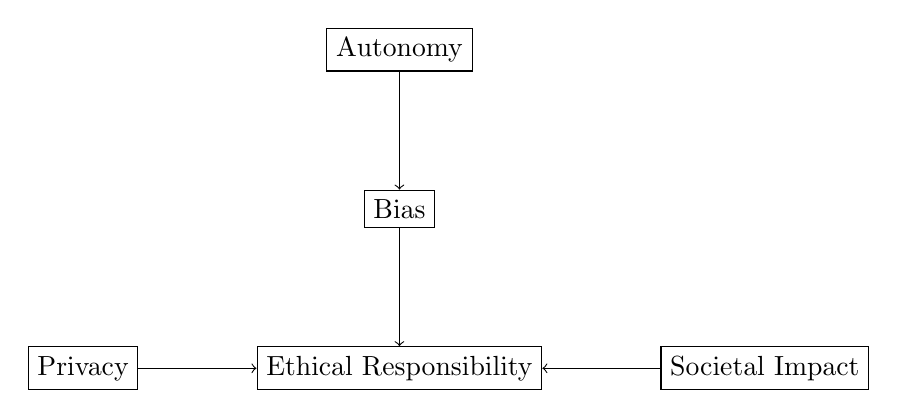
\begin{tikzpicture}[node distance=1.5cm]
            \node (autonomy) [draw] {Autonomy};
            \node (bias) [draw, below=of autonomy] {Bias};
            \node (responsibility) [draw, below=of bias] {Ethical Responsibility};
            \node (privacy) [draw, left=of responsibility] {Privacy};
            \node (societal) [draw, right=of responsibility] {Societal Impact};

            \path[->] (autonomy) edge (bias);
            \path[->] (bias) edge (responsibility);
            \path[->] (privacy) edge (responsibility);
            \path[->] (societal) edge (responsibility);
        \end{tikzpicture}
        \caption{Key Ethical Areas in MARL}
    \end{figure}
\end{frame}

\begin{frame}[fragile]
    \frametitle{Conclusion}
    As we develop and integrate Multi-Agent Reinforcement Learning systems, it is crucial to address ethical implications. 
    Collaboration among researchers, developers, and policymakers is needed to establish responsible AI that contributes positively to society while minimizing harm.
\end{frame}

\begin{frame}[fragile]
    \frametitle{Research Trends in Multi-Agent Reinforcement Learning}
    \begin{block}{Introduction}
        Multi-Agent Reinforcement Learning (MARL) is gaining traction as researchers seek to develop robust algorithms that enable multiple agents to learn and collaborate (or compete) in complex environments. This presentation discusses emerging research areas and future directions in MARL.
    \end{block}
\end{frame}

\begin{frame}[fragile]
    \frametitle{Decentralized Learning and Coordination}
    \begin{itemize}
        \item \textbf{Concept:} In decentralized structures, agents learn independently while still coordinating their actions to achieve a common goal.
        \item \textbf{Example:} Traffic management systems where individual vehicles (agents) decide routes based on their local observations while optimizing overall traffic flow.
    \end{itemize}
\end{frame}

\begin{frame}[fragile]
    \frametitle{Scalability in Multi-Agent Systems}
    \begin{itemize}
        \item \textbf{Concept:} Research focuses on making MARL algorithms scalable to handle large numbers of agents effectively.
        \item \textbf{Example:} Expanding game environments like StarCraft or complex simulations where hundreds of agents need to operate without significant degradation in performance.
    \end{itemize}
\end{frame}

\begin{frame}[fragile]
    \frametitle{Communication and Negotiation Strategies}
    \begin{itemize}
        \item \textbf{Concept:} Agents develop effective communication protocols and negotiation tactics to better coordinate actions.
        \item \textbf{Example:} In a trading scenario, agents might negotiate prices or resource allocation to maximize their utility.
    \end{itemize}
\end{frame}

\begin{frame}[fragile]
    \frametitle{Robustness and Safety in MARL}
    \begin{itemize}
        \item \textbf{Concept:} Focusing on how agents can learn in uncertain or adversarial environments while maintaining performance, safety, and ethical outcomes.
        \item \textbf{Example:} Autonomous drones collaborating in search and rescue missions must ensure safe interaction to avoid collisions while maximizing coverage area.
    \end{itemize}
\end{frame}

\begin{frame}[fragile]
    \frametitle{Transfer Learning and Domain Adaptation}
    \begin{itemize}
        \item \textbf{Concept:} Techniques that facilitate the transfer of knowledge between tasks or environments, improving learning efficiency.
        \item \textbf{Example:} An agent trained in one game (e.g., a simplified version of chess) using that knowledge when learning another, more complex version of the game.
    \end{itemize}
\end{frame}

\begin{frame}[fragile]
    \frametitle{Theoretical Foundations and Evaluation Metrics}
    \begin{itemize}
        \item \textbf{Concept:} Researchers are trying to establish solid theoretical foundations for MARL to better understand its principles and outcomes.
        \item \textbf{Example:} Developing new metrics to assess cooperation and competition levels among agents can provide insights into system performance beyond simple rewards.
    \end{itemize}
\end{frame}

\begin{frame}[fragile]
    \frametitle{Key Takeaways}
    \begin{itemize}
        \item The field of MARL is evolving to address communication, scalability, safety, and effective coordination among agents.
        \item Practical applications extend across industries from autonomous vehicles to resource management, positioning MARL as a critical area for future research and development.
    \end{itemize}
\end{frame}

\begin{frame}[fragile]
    \frametitle{Conclusion}
    Emerging trends in MARL open the door to exciting research opportunities and applications, necessitating continuous exploration and innovation to address the challenges and complexities inherent to multi-agent environments.

    \begin{block}{Next Steps}
        Ensure to connect this discussion with hands-on implementation insights, as understanding these trends will inform practical applications in the field.
    \end{block}
\end{frame}

\begin{frame}[fragile]
    \frametitle{Hands-on Workshop: Implementing Multi-Agent Systems}
    
    \begin{block}{Interactive Session Overview}
        In this session, we will explore how to implement a simple Multi-Agent Reinforcement Learning (MARL) system. This hands-on workshop will engage you in practical coding exercises and simulations that embody the core concepts of MARL.
    \end{block}
\end{frame}

\begin{frame}[fragile]
    \frametitle{Key Concepts}
    
    \begin{enumerate}
        \item \textbf{Multi-Agent System (MAS)}:
            \begin{itemize}
                \item A computational system where multiple agents interact in an environment.
                \item Each agent has its own goals and learning mechanisms.
                \item \textbf{Example}: Autonomous vehicles coordinating their paths at an intersection.
            \end{itemize}
        
        \item \textbf{Reinforcement Learning (RL)}:
            \begin{itemize}
                \item A learning paradigm where agents take actions in an environment to maximize cumulative reward.
                \item \textbf{Key Components}:
                    \begin{itemize}
                        \item \textbf{Agent}: Learns and makes decisions.
                        \item \textbf{Environment}: The context in which agents operate.
                        \item \textbf{Actions (A)}: Possible moves the agent can make.
                        \item \textbf{Rewards (R)}: Feedback guiding the agent's learning.
                    \end{itemize}
            \end{itemize}
        
        \item \textbf{Collaboration vs. Competition}:
            \begin{itemize}
                \item Agents can collaborate to achieve a common goal (e.g. resource allocation).
                \item Alternatively, they may compete against each other (e.g. games like Chess or Go).
            \end{itemize}
    \end{enumerate}
\end{frame}

\begin{frame}[fragile]
    \frametitle{Workshop Outline}
    
    \begin{enumerate}
        \item \textbf{Setup the Environment}:
            \begin{itemize}
                \item Use Python with libraries such as OpenAI Gym and NumPy.
                \item Install necessary packages:
                \begin{lstlisting}[language=bash]
pip install gym numpy
                \end{lstlisting}
            \end{itemize}

        \item \textbf{Define the Multi-Agent Environment}:
            \begin{itemize}
                \item Use a simple grid environment or a standard one from OpenAI Gym that supports multiple agents.
                \item \textbf{Example}: A cooperative grid-world where agents need to reach designated targets.
            \end{itemize}

        \item \textbf{Coding the Agents}:
            \begin{itemize}
                \item Implement a Q-learning algorithm for each agent.
                \item \textbf{Key Code Snippet}:
                \begin{lstlisting}[language=python]
import numpy as np

class QLearningAgent:
    def __init__(self, learning_rate=0.1, discount_factor=0.9):
        self.q_table = np.zeros((state_space_size, action_space_size))
        self.learning_rate = learning_rate
        self.discount_factor = discount_factor

    def update_q_value(self, state, action, reward, next_state):
        best_next_action = np.argmax(self.q_table[next_state])
        self.q_table[state, action] += self.learning_rate * (reward + self.discount_factor * self.q_table[next_state, best_next_action] - self.q_table[state, action])
                \end{lstlisting}
            \end{itemize}
    \end{enumerate}
\end{frame}

\begin{frame}[fragile]
    \frametitle{Key Points to Emphasize}
    
    \begin{itemize}
        \item \textbf{Importance of Communication}: In collaborative settings, how agents share information can significantly impact performance.
        \item \textbf{Exploration vs. Exploitation}: Highlight how agents balance exploring new strategies against exploiting known rewarding actions.
        \item \textbf{Scalability}: Discuss the challenges of scaling up the number of agents.
    \end{itemize}
    
    \begin{block}{Wrap-Up}
        This workshop serves as a foundational exercise in understanding the dynamics of Multi-Agent Reinforcement Learning. By actively participating, you will gain insights into the complexities and implementation challenges inherent in these systems, setting the stage for future research and practical applications.
    \end{block}
\end{frame}

\begin{frame}[fragile]
    \frametitle{Next Steps}
    
    \begin{block}{Prepare for Next Slide}
        Next, we will cover "Collaboration Skills in Group Projects" to learn how to effectively work in teams for MARL research.
    \end{block}
    
    \begin{block}{Questions}
        Feel free to ask any questions or seek clarifications as we move through the hands-on implementation!
    \end{block}
\end{frame}

\begin{frame}[fragile]
    \frametitle{Collaboration Skills in Group Projects - Introduction}
    \begin{block}{Overview}
        Effective teamwork is essential in multi-agent reinforcement learning (MARL) research projects, where diverse skills and perspectives converge to tackle complex problems.
    \end{block}
    \begin{block}{Benefits of Collaboration}
        Collaboration can enhance:
        \begin{itemize}
            \item Creativity
            \item Productivity
            \item Innovative Solutions
        \end{itemize}
    \end{block}
\end{frame}

\begin{frame}[fragile]
    \frametitle{Collaboration Skills in Group Projects - Key Guidelines}
    \begin{enumerate}
        \item \textbf{Clear Communication}
        \begin{itemize}
            \item \textbf{Concept}: Establish open lines of communication to ensure everyone is aligned.
            \item \textbf{Practice}: Use project management tools (e.g., Slack, Trello).
            \item \textbf{Example}: Schedule weekly stand-up meetings for progress updates.
        \end{itemize}

        \item \textbf{Defined Roles and Responsibilities}
        \begin{itemize}
            \item \textbf{Concept}: Assign roles based on each member’s strengths.
            \item \textbf{Practice}: Define tasks clearly.
            \item \textbf{Example}: One member focuses on algorithm design, another on simulation environments.
        \end{itemize}
        
        \item \textbf{Collaborative Problem Solving}
        \begin{itemize}
            \item \textbf{Concept}: Encourage brainstorming and collective decision-making.
            \item \textbf{Practice}: Use “round-robin brainstorming”.
            \item \textbf{Example}: Discuss potential solutions for convergence issues.
        \end{itemize}
    \end{enumerate}
\end{frame}

\begin{frame}[fragile]
    \frametitle{Collaboration Skills in Group Projects - More Guidelines}
    \begin{enumerate}[resume]
        \item \textbf{Regular Feedback and Iteration}
        \begin{itemize}
            \item \textbf{Concept}: Implement an iterative review process.
            \item \textbf{Practice}: Set up bi-weekly reviews.
            \item \textbf{Example}: Gather feedback after model training iterations.
        \end{itemize}

        \item \textbf{Conflict Resolution}
        \begin{itemize}
            \item \textbf{Concept}: Address conflicts promptly and constructively.
            \item \textbf{Practice}: Foster a comfortable environment for concerns.
            \item \textbf{Example}: Discuss evidence and rationale supporting each model choice.
        \end{itemize}
        
        \item \textbf{Documentation and Sharing Knowledge}
        \begin{itemize}
            \item \textbf{Concept}: Maintain thorough documentation of the project's progress.
            \item \textbf{Practice}: Use shared documents for capturing insights.
            \item \textbf{Example}: Create a repository for code and reports.
        \end{itemize}
    \end{enumerate}
\end{frame}

\begin{frame}[fragile]
    \frametitle{Collaboration Skills in Group Projects - Summary}
    \begin{block}{Key Takeaways}
        - Collaboration in MARL requires commitment from all team members.
        - Focus on communication, roles, problem-solving, and feedback.
    \end{block}
    \begin{block}{Final Thoughts}
        A successful group project is about both the outcome and growing as a team.
    \end{block}
\end{frame}

\begin{frame}[fragile]
    \frametitle{Collaboration Skills in Group Projects - Code Snippet}
    \begin{lstlisting}[language=Python]
for agent in agents:
    action = agent.select_action(state)  # Each agent decides an action
    new_state, reward, done = environment.step(action)  # Interact with the environment
    agent.learn(state, action, reward, new_state)  # Learn from the experience
    \end{lstlisting}
\end{frame}

\begin{frame}
    \frametitle{Student Presentations on RL Research}
    \begin{block}{Overview of Presentation Format}
        \textbf{Objective:} Each student will present their research focusing on Multi-Agent Reinforcement Learning (MARL). This session aims to share insights, methodologies, and findings, fostering a collaborative learning environment.
    \end{block}
\end{frame}

\begin{frame}
    \frametitle{Presentation Structure}
    \begin{enumerate}
        \item \textbf{Introduction (1-2 minutes)}
            \begin{itemize}
                \item Briefly introduce the research topic and its relevance to MARL.
                \item State your research question or hypothesis.
            \end{itemize}
        \item \textbf{Background (2-3 minutes)}
            \begin{itemize}
                \item What is Multi-Agent Reinforcement Learning?
                \item How it differs from single-agent RL.
                \item Key terms: agents, environment, policies, rewards, etc.
                \item Significant prior work and foundational theories.
            \end{itemize}
        \item \textbf{Methodology (3-4 minutes)}
            \begin{itemize}
                \item Describe your approach:
                \begin{itemize}
                    \item Model Used: (e.g., Q-Learning, A3C, DDPG)
                    \item Environment: Details about the simulation or real-world setting.
                    \item Agent Interaction: How agents communicate and collaborate.
                \end{itemize}
            \end{itemize}
    \end{enumerate}
\end{frame}

\begin{frame}[fragile]
    \frametitle{Methodology Continued}
    \begin{itemize}
        \item Include any relevant algorithms or frameworks.
        \item Example code snippet (optional):
        \begin{lstlisting}[language=Python]
class MultiAgentEnv(gym.Env):
    def __init__(self):
        self.agents = [Agent(i) for i in range(num_agents)]
    # Add more methods here
        \end{lstlisting}
    \end{itemize}
\end{frame}

\begin{frame}
    \frametitle{Results and Conclusions}
    \begin{itemize}
        \item \textbf{Results (3-4 minutes)}
            \begin{itemize}
                \item Present your findings clearly with graphs and charts.
                \item Compare results with existing benchmarks.
                \item Discuss unexpected outcomes and implications.
            \end{itemize}
        \item \textbf{Conclusion (2-3 minutes)}
            \begin{itemize}
                \item Summarize key takeaways from your research.
                \item Discuss practical implications or future directions in MARL research.
            \end{itemize}
    \end{itemize}
\end{frame}

\begin{frame}
    \frametitle{Engagement and Assessment}
    \begin{itemize}
        \item \textbf{Q\&A Session (2-3 minutes)}
            \begin{itemize}
                \item Encourage audience questions for clarity and engagement.
            \end{itemize}
        \item \textbf{Key Points to Emphasize}
            \begin{itemize}
                \item Collaborative Nature of MARL and impact of communication.
                \item Ethical considerations in MARL applications.
            \end{itemize}
        \item \textbf{Assessment Criteria}
            \begin{itemize}
                \item Clarity of presentation.
                \item Depth of research.
                \item Engagement with the audience.
            \end{itemize}
    \end{itemize}
\end{frame}

\begin{frame}
    \frametitle{Tips for an Engaging Presentation}
    \begin{itemize}
        \item Use Visuals: Incorporate diagrams to explain agent interactions.
        \item Real-World Examples: Connect research to real-life applications.
        \item Practice Delivery: Rehearse to ensure clarity and timing.
    \end{itemize}
\end{frame}

\begin{frame}[fragile]
    \frametitle{Assessments and Evaluation in Multi-Agent Reinforcement Learning}
    \begin{block}{Overview}
        Evaluating Multi-Agent Reinforcement Learning (MARL) projects is critical for understanding the effectiveness and efficiency of algorithms in complex environments. This slide provides an overview of various assessment methods, key criteria, and practical examples to guide students in presenting and evaluating their work in MARL.
    \end{block}
\end{frame}

\begin{frame}[fragile]
    \frametitle{Key Assessment Methods - Part 1}
    \begin{enumerate}
        \item \textbf{Performance Metrics}:
            \begin{itemize}
                \item \textbf{Cumulative Reward}:
                    \begin{itemize}
                        \item Measure the total reward collected by agents over episodes. Useful for understanding overall success.
                        \item \textit{Example:} In a cooperative setting, an increase in cumulative reward indicates successful collaboration.
                    \end{itemize}
                \item \textbf{Success Rate}:
                    \begin{itemize}
                        \item The percentage of episodes where certain objectives are met.
                        \item \textit{Example:} In a multi-agent navigation scenario, success rate reflects how often all agents reach a target location.
                    \end{itemize}
            \end{itemize}
        
        \item \textbf{Learning Speed}:
            \begin{itemize}
                \item \textbf{Convergence Rate}: The speed at which agents reach optimal policies.
                \item \textit{Example:} A plot of cumulative reward against episodes can illustrate convergence behavior.
            \end{itemize}
    \end{enumerate}
\end{frame}

\begin{frame}[fragile]
    \frametitle{Key Assessment Methods - Part 2}
    \begin{enumerate}
        \setcounter{enumi}{2} % Continue numbering
        \item \textbf{Scalability}:
            \begin{itemize}
                \item Assess how well the algorithms perform as the number of agents or complexity of the environment increases.
                \item \textit{Example:} Testing the system with varying numbers of agents (2, 5, 10) on the same task.
            \end{itemize}

        \item \textbf{Robustness}:
            \begin{itemize}
                \item Evaluate how agents perform under varying environmental conditions or disturbances.
                \item \textit{Example:} Introducing random obstacles in a pathfinding task to see if agents can still reach the target.
            \end{itemize}
    \end{enumerate}
\end{frame}

\begin{frame}[fragile]
    \frametitle{Presentation Evaluation Criteria}
    When presenting MARL projects, assess the following aspects:
    
    \begin{enumerate}
        \item \textbf{Clarity and Structure}:
            \begin{itemize}
                \item Is the project clearly articulated with logical flow?
                \item \textit{Tips:} Begin with a problem statement, methodology, results, and conclusion.
            \end{itemize}
        
        \item \textbf{Technical Depth}:
            \begin{itemize}
                \item Are the concepts well-explained and backed by theoretical foundations?
                \item \textit{Tips:} Use relevant equations or algorithms, such as Q-learning or Policy Gradient methods.
            \end{itemize}
        
        \item \textbf{Innovativeness}:
            \begin{itemize}
                \item Does the project propose novel methods or applications in MARL?
            \end{itemize}
        
        \item \textbf{Results and Discussion}:
            \begin{itemize}
                \item Are the results clearly presented (charts, graphs) with thorough evaluation of the findings?
            \end{itemize}
    \end{enumerate}
\end{frame}

\begin{frame}[fragile]
    \frametitle{Example of Metrics Presentation}
    \begin{itemize}
        \item \textbf{Cumulative Reward vs. Episode Graph}:
            \begin{itemize}
                \item Use line graphs to show reward fluctuations across training episodes for individual agents.
            \end{itemize}
        
        \item \textbf{Success Rate Table}:
            \begin{table}[ht]
                \centering
                \begin{tabular}{|c|c|}
                    \hline
                    \textbf{Number of Agents} & \textbf{Success Rate (\%)} \\
                    \hline
                    2 & 85 \\
                    5 & 70 \\
                    10 & 55 \\
                    \hline
                \end{tabular}
                \caption{Success Rates for Varying Number of Agents}
            \end{table}
    \end{itemize}
\end{frame}

\begin{frame}[fragile]
    \frametitle{Conclusion and Key Takeaways}
    Assessments in multi-agent reinforcement learning involve:
    \begin{itemize}
        \item Quantitative metrics on performance, 
        \item Qualitative feedback on presentations, 
        \item Comprehensive examination of results.
    \end{itemize}

    \textbf{Remember:}
    \begin{itemize}
        \item Focus on both performance and presentation quality.
        \item Leverage visual aids to enhance understanding.
        \item Encourage peer feedback to foster collaborative learning.
    \end{itemize}
\end{frame}

\begin{frame}[fragile]
    \frametitle{Feedback Mechanisms for Collaborative Projects - Overview}
    Effective feedback mechanisms are crucial in collaborative projects, particularly in multi-agent systems like Reinforcement Learning (RL). They:
    \begin{itemize}
        \item Facilitate communication
        \item Enhance learning
        \item Ensure productive contributions
    \end{itemize}
    The main types include:
    \begin{enumerate}
        \item \textbf{Feedback Loops}: Continuous cycles of evaluation and improvement.
        \item \textbf{Peer Evaluations}: Structured assessments by team members.
    \end{enumerate}
\end{frame}

\begin{frame}[fragile]
    \frametitle{Feedback Mechanisms for Collaborative Projects - Importance}
    The importance of feedback mechanisms includes:
    \begin{itemize}
        \item \textbf{Enhances Performance}: Provides insights into strengths and weaknesses.
        \item \textbf{Encourages Engagement}: Increases member involvement due to reciprocal feedback.
        \item \textbf{Builds Trust}: Promotes a culture of transparency and trust.
    \end{itemize}
\end{frame}

\begin{frame}[fragile]
    \frametitle{Feedback Mechanisms for Collaborative Projects - Implementation}
    Implement effective feedback through:
    \begin{enumerate}
        \item \textbf{Set Clear Expectations}: Define feedback types and frequency.
        \item \textbf{Use Rubrics}: Standardize peer evaluations for objectivity.
        \item \textbf{Foster a Growth Mindset}: Encourage viewing feedback as a tool for growth.
    \end{enumerate}
    \begin{block}{Conclusion}
        Effective feedback maximizes learning and mirrors adaptive processes in RL, aligning team members toward success and cohesion.
    \end{block}
\end{frame}

\begin{frame}
    \frametitle{Course Wrap-up and Key Takeaways}
    In this session, we summarize the key concepts learned in Multi-Agent Reinforcement Learning (MARL) and their applications.
\end{frame}

\begin{frame}
    \frametitle{Understanding Multi-Agent Reinforcement Learning (MARL)}
    \begin{itemize}
        \item Multi-Agent Reinforcement Learning (MARL) extends traditional RL with multiple agents in a shared environment.
        \item Key distinctions:
        \begin{itemize}
            \item \textbf{Cooperation vs. Competition}: Agents can collaborate or compete for resources.
            \item \textbf{Decentralized Learning}: Agents update their strategies based on individual experiences, leading to emergent behaviors.
        \end{itemize}
    \end{itemize}
\end{frame}

\begin{frame}
    \frametitle{Key Concepts Explored}
    \begin{itemize}
        \item \textbf{Agent-environment Interaction}: Agents take actions and receive feedback, influencing future decisions.
        \item \textbf{Joint Action Learning}: Agents learn from both their own and others' actions, requiring consideration of peers' strategies.
    \end{itemize}
\end{frame}

\begin{frame}
    \frametitle{Collaboration Mechanisms}
    Exploring cooperative strategies:
    \begin{itemize}
        \item \textbf{Shared Rewards}: Collective rewards encourage collaboration among agents.
        \item \textbf{Communication}: Information exchange enhances performance, necessitating effective message-sharing mechanisms.
    \end{itemize}
\end{frame}

\begin{frame}
    \frametitle{Practical Applications of MARL}
    \begin{itemize}
        \item \textbf{Robotics}: Collaborative robots (cobots) in warehouse automation.
        \item \textbf{Traffic Management}: Self-driving cars synchronizing through communication.
        \item \textbf{Gaming}: Intelligent NPCs collaborating or competing in complex games.
    \end{itemize}
\end{frame}

\begin{frame}[fragile]
    \frametitle{Key Algorithms and Techniques}
    \begin{itemize}
        \item \textbf{Q-Learning Extensions}: 
        \begin{itemize}
            \item Centralized Training with Decentralized Execution (CTDE) enables shared training data while preserving independent decision-making during execution.
        \end{itemize}
    \end{itemize}
    
    \begin{block}{Example Code Snippet: Q-Learning Update Rule}
    \begin{lstlisting}[language=Python]
# Q-learning update formula for an agent
Q[state, action] += learning_rate * (reward + discount_factor * max(Q[next_state, all_actions]) - Q[state, action])
    \end{lstlisting}
    \end{block}
\end{frame}

\begin{frame}
    \frametitle{Important Metrics for Evaluation}
    When assessing MARL systems, consider:
    \begin{itemize}
        \item \textbf{Cumulative Reward}: Total returns obtained over time.
        \item \textbf{Convergence}: Speed and reliability of reaching an optimal strategy.
    \end{itemize}
\end{frame}

\begin{frame}
    \frametitle{Challenges Ahead}
    Key difficulties include:
    \begin{itemize}
        \item \textbf{Scalability}: Performance declines with an increasing number of agents.
        \item \textbf{Non-stationarity}: The environment evolves as agents learn, complicating strategy formulation.
    \end{itemize}
\end{frame}

\begin{frame}
    \frametitle{Conclusion}
    Mastering MARL concepts is essential for creating systems solving complex collective intelligence problems. Understanding these principles enables innovative applications for improved collaboration and efficiency across diverse domains.
    \begin{block}{Reminder for Discussion}
        Prepare any questions for the upcoming Q\&A session to enhance understanding!
    \end{block}
\end{frame}

\begin{frame}[fragile]
    \frametitle{Q\&A Session on Multi-Agent Reinforcement Learning}
    % Overview of this session
    \begin{block}{Overview}
        This slide provides an opportunity for participants to engage in an open discussion 
        regarding Multi-Agent Reinforcement Learning (MARL). This collaborative learning 
        approach can help deepen understanding and address specific questions about the 
        concepts covered in this week's material.
    \end{block}
\end{frame}

\begin{frame}[fragile]
    \frametitle{Key Concepts in MARL}
    % Key concepts to consider
    \begin{enumerate}
        \item \textbf{Definition of Multi-Agent Reinforcement Learning}:
        \begin{itemize}
            \item A subfield where multiple agents interact within an environment to learn optimal behaviors.
            \item Agents learn from both their actions and the actions of others.
        \end{itemize}
        
        \item \textbf{Types of Multi-Agent Systems}:
        \begin{itemize}
            \item \textbf{Cooperative}: Agents work together (e.g., autonomous vehicles).
            \item \textbf{Competitive}: Agents compete against each other (e.g., games).
            \item \textbf{Mixed}: Combination of cooperation and competition (e.g., economic markets).
        \end{itemize}
        
        \item \textbf{Challenges in MARL}:
        \begin{itemize}
            \item \textbf{Non-Stationarity}: Agents influence each other's learning.
            \item \textbf{Scalability}: Complexity increases with the number of agents.
            \item \textbf{Credit Assignment Problem}: Identifying which agent's actions lead to rewards.
        \end{itemize}
    \end{enumerate}
\end{frame}

\begin{frame}[fragile]
    \frametitle{Discussion Points in MARL}
    % Points for discussion
    \begin{block}{Discussion Points}
        \begin{itemize}
            \item How do different learning algorithms adapt for multiple agents?
            \item What strategies mitigate the non-stationarity problem in learning?
            \item Can you provide real-world examples successfully using MARL?
            \item How does agent communication play a role in collaborative tasks?
        \end{itemize}
    \end{block}

    \begin{block}{Example Applications}
        \begin{itemize}
            \item \textbf{Robotic Swarms}: Drones coordinating for search and rescue.
            \item \textbf{Multi-Player Gaming}: Evolving strategies in real-time games.
            \item \textbf{Traffic Management}: Vehicles optimizing routes and timings.
        \end{itemize}
    \end{block}

    \begin{block}{Invitation for Questions}
        Encourage participants to ask questions about the topics covered, including challenges to explore further.
    \end{block}
\end{frame}

\begin{frame}[fragile]
    \frametitle{Resources for Further Learning - Overview}
    \begin{block}{Overview}
    Multi-Agent Reinforcement Learning (MARL) encompasses various techniques and concepts that can be challenging yet rewarding to explore. The following resources provide an opportunity for deeper engagement and understanding of MARL concepts, methodologies, and applications.
    \end{block}
\end{frame}

\begin{frame}[fragile]
    \frametitle{Resources for Further Learning - Recommended Readings}
    \begin{enumerate}
        \item \textbf{Book:} 
        \begin{itemize}
            \item \textit{"Multi-Agent Reinforcement Learning: A Review"}
            \item \textbf{Authors:} Busoniu, L., B. De Schutter, and D. Ernst
            \item \textbf{Link:} \url{https://link.springer.com/chapter/10.1007/978-3-540-30225-8_1}
            \item This comprehensive review outlines key concepts, challenges, and open research questions in MARL.
        \end{itemize}
        
        \item \textbf{Research Paper:}
        \begin{itemize}
            \item \textit{"Cooperative Multi-Agent Reinforcement Learning with Emergent Communication"}
            \item \textbf{Authors:} Mordatch, I. and Abbeel, P.
            \item \textbf{Link:} \url{https://arxiv.org/abs/1703.04960}
            \item This paper discusses how agents can develop communication strategies to enhance learning efficiency in cooperative tasks.
        \end{itemize}
        
        \item \textbf{Online Course:}
        \begin{itemize}
            \item \textit{"Deep Reinforcement Learning Nanodegree"}
            \item \textbf{Link:} \url{https://www.udacity.com/course/deep-reinforcement-learning-nanodegree--nd893}
            \item Offered on Udacity, this course includes modules specifically focusing on multi-agent scenarios.
        \end{itemize}
    \end{enumerate}
\end{frame}

\begin{frame}[fragile]
    \frametitle{Resources for Further Learning - Tools and Key Points}
    \begin{block}{Online Resources and Tools}
    \begin{itemize}
        \item \textbf{OpenAI Gym:} A toolkit for developing and comparing RL agents. \url{https://gym.openai.com/}
        \item \textbf{MPE:} Multi-Agent Particle Environments for testing algorithms. \url{https://github.com/openai/multiagent-particle-envs}
    \end{itemize}
    \end{block}

    \begin{block}{Key Points to Emphasize}
    \begin{itemize}
        \item Collaboration vs. Competition: Understand the dynamics between cooperating and competing agents in MARL scenarios.
        \item Communication: Explore how agents can communicate and how this affects their learning outcomes.
        \item Emergent Behavior: Study how individual agent behaviors can lead to complex group dynamics.
    \end{itemize}
    \end{block}
\end{frame}

\begin{frame}[fragile]
    \frametitle{Example Code Snippet - Multi-Agent Environment}
    \begin{lstlisting}[language=Python]
import gym
from stable_baselines3 import PPO

# Create multi-agent environment
env = gym.make("MultiAgentEnvironment-v0")  # Replace with actual env

# Initialize the agent
agent = PPO("MlpPolicy", env, verbose=1)

# Train the agent
agent.learn(total_timesteps=20000)
    \end{lstlisting}
\end{frame}

\begin{frame}[fragile]
    \frametitle{Resources for Further Learning - Conclusion}
    \begin{block}{Conclusion}
    Exploring these resources will enhance your understanding of multi-agent scenarios and equip you with the knowledge necessary to implement MARL techniques effectively. Engaging with research papers, online courses, and practical environments will solidify your learning and spark innovation in your projects.
    \end{block}
\end{frame}

\begin{frame}[fragile]
    \frametitle{Important Dates and Deadlines - Overview}
    \begin{block}{Overview}
        In the context of Multi-Agent Reinforcement Learning, staying up to date with assignments and project deadlines is critical for your success in this course. Proper time management will enhance your understanding of the material and improve your final outcomes. 
        This slide outlines the important dates you should keep in mind.
    \end{block}
\end{frame}

\begin{frame}[fragile]
    \frametitle{Important Dates and Deadlines - Key Deadlines}
    \begin{enumerate}
        \item \textbf{Assignment 3: Multi-Agent Policy Gradient Implementation}\\
        \textit{Due Date: March 15, 2024}\\
        \textbf{Description:} Implement a policy gradient algorithm for agents working collaboratively in a simulated environment.\\
        \textbf{Key Points:}
        \begin{itemize}
            \item Review the implementation guidelines provided in the course materials.
            \item Focus on optimizing the agents’ learning strategies.
            \item Ensure to test and benchmark performance.
        \end{itemize}

        \item \textbf{Midterm Project: Evaluating Collaborative vs. Competing Agents}\\
        \textit{Due Date: April 10, 2024}\\
        \textbf{Description:} Analyze and report on the results of scenarios where agents either cooperate or compete.\\
        \textbf{Key Points:}
        \begin{itemize}
            \item Aim to depict clear comparisons with graphs illustrating success metrics.
            \item Make use of the simulation frameworks discussed in Week 5.
            \item Submit a draft by April 1, 2024, for feedback.
        \end{itemize}

        \item \textbf{Final Examination on Multi-Agent Systems}\\
        \textit{Exam Date: April 25, 2024}\\
        \textbf{Description:} Comprehensive exam covering all aspects of multi-agent reinforcement learning, including theoretical and practical knowledge.\\
        \textbf{Preparation Tips:}
        \begin{itemize}
            \item Review lecture notes and resources provided in Week 9.
            \item Form study groups to discuss concepts and solve example problems.
            \item Practice past exam papers and questions related to multi-agent dynamics.
        \end{itemize}
    \end{enumerate}
\end{frame}

\begin{frame}[fragile]
    \frametitle{Important Dates and Deadlines - Final Notes}
    \begin{block}{Final Notes}
        \begin{itemize}
            \item \textbf{Communication:} Regularly check announcements on the course platform for any changes in deadlines.
            \item \textbf{Time Management:} Start early; don’t wait until the last minute to work on your assignments and projects.
            \item \textbf{Support:} If you have questions or require assistance, reach out to your instructor during office hours or via email.
        \end{itemize}
    \end{block}
    
    \begin{block}{Summary}
        Keep this slide as a reference throughout the course to remain informed and prepared for the upcoming challenges. Your proactive approach will ensure a rewarding learning experience in multi-agent systems!
    \end{block}
\end{frame}

\begin{frame}[fragile]
    \frametitle{Conclusion and Next Steps - Summary of Key Concepts}
    \begin{itemize}
        \item \textbf{Definition of MARL:} Involves multiple agents learning simultaneously and interacting with one another.
        \item \textbf{Key Challenges:} Non-stationarity, credit assignment, and communication protocols affect learning and adaptation.
        \item \textbf{Common Algorithms:} Familiarize with MADDPG and COMA for handling multi-agent interactions.
    \end{itemize}
\end{frame}

\begin{frame}[fragile]
    \frametitle{Conclusion and Next Steps - What to Expect}
    \begin{enumerate}
        \item \textbf{Advanced Algorithms:} Explore softmax policies and value-decomposition techniques in MARL.
        \item \textbf{Simulation Environments:} Learning implementation of MARL using OpenAI Gym or Unity ML-Agents.
        \item \textbf{Real-World Applications:} Case studies in robotics, finance, and autonomous vehicles to contextualize learning.
        \item \textbf{Collaborative Project:} Design a MARL system tailored to a specific problem.
    \end{enumerate}
\end{frame}

\begin{frame}[fragile]
    \frametitle{Conclusion and Next Steps - Preparation Tips and Key Takeaways}
    \begin{block}{Preparation Tips}
        \begin{itemize}
            \item Review materials related to MARL concepts.
            \item Start coding basic implementations of MARL algorithms in Python.
            \item Engage in discussions with peers and form study groups.
            \item Set milestones for group project research and coding phases.
        \end{itemize}
    \end{block}
    
    \begin{block}{Key Takeaways}
        \begin{itemize}
            \item Understand collaborative and competitive nature of MARL.
            \item Prepare for implementing algorithms in simulation environments.
            \item Engage actively in discussions and projects for deeper learning.
        \end{itemize}
    \end{block}
\end{frame}


\end{document}